\chapter{Introduction}
\label{chap:intro}

\begin{figure}
\caption{The Internet's four-layer model}
\label{f:stack}
\begin{centering}
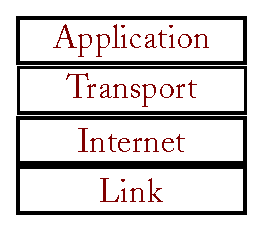
\includegraphics{layers.pdf}

\end{centering}
\end{figure}

\begin{figure}
\caption{As the Internet has evolved, researchers have created at
  least 40 mechanisms to govern resource allocation on the
  network---both entirely distributed schemes (``end-to-end'') and
  ones that include code running ``in-net.''}
\label{f:march}

\vspace{\baselineskip}

\begin{centering}
\noindent 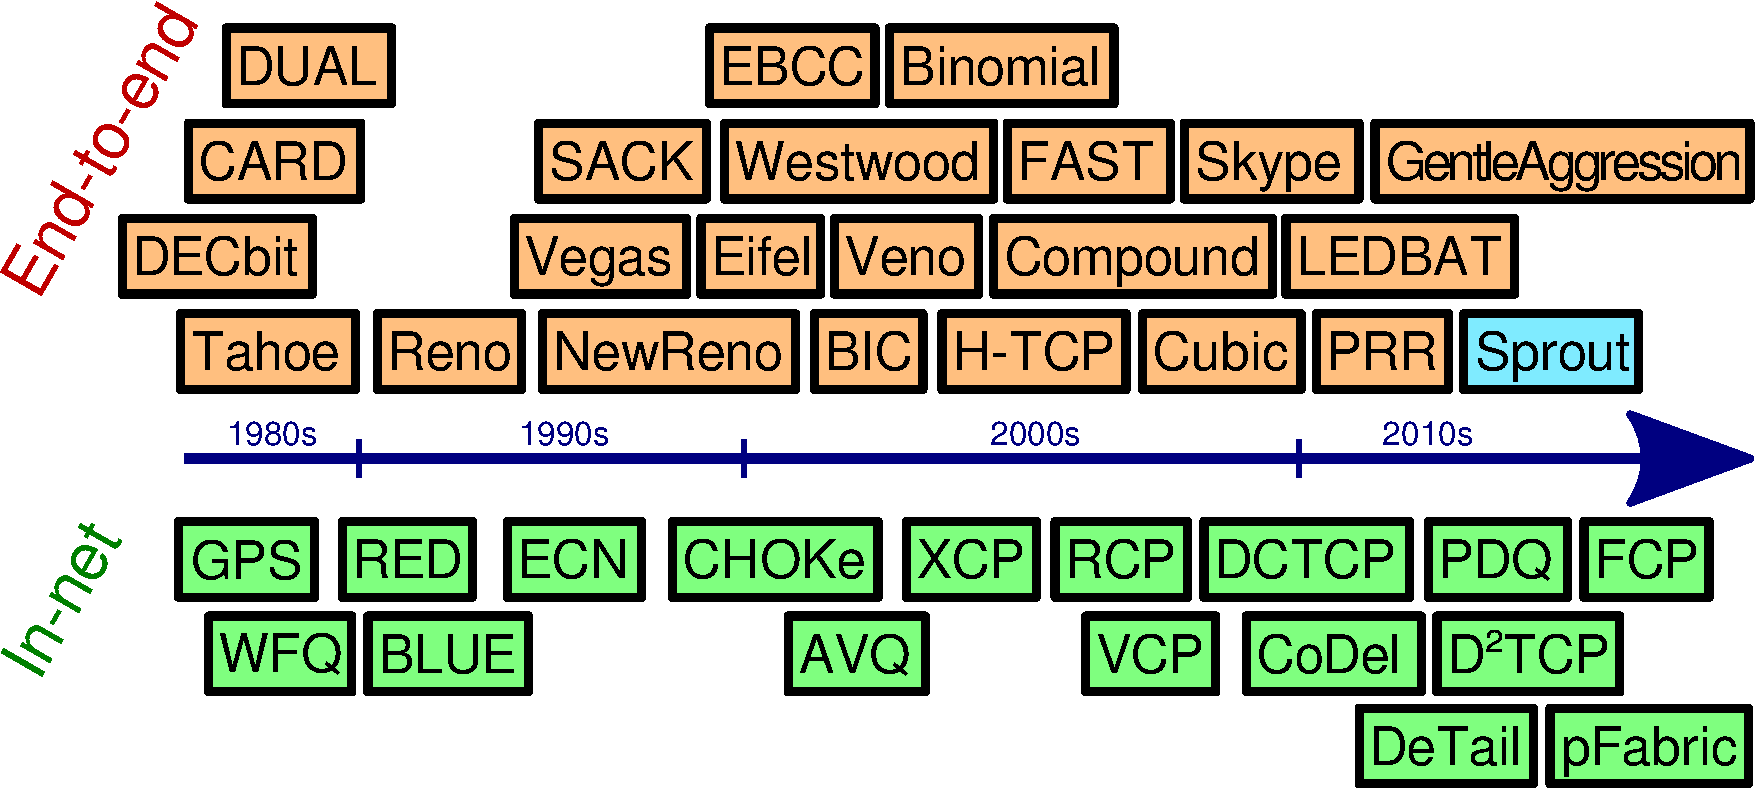
\includegraphics[width=\textwidth]{march2-all.pdf}

\end{centering}
\end{figure}

Over the last 25 years, the Internet has transformed from an academic
networking experiment into a global utility with billions of
users. As part of this transformation, every layer of the Internet
``stack'' has seen dramatic change.

At the link layer, technologies that did not exist 25 years
ago now dominate---including wireless local-area networks (Wi-Fi),
cellular networks, datacenter interconnects, and transoceanic links
with high delay.

One layer up, at the Internet layer, mobility is now
ubiquitous. User devices regularly change their interface IP addresses
as they roam from network to network.

At the top layer of the Internet stack---the application
layer---none of the dominant applications of today existed 25 years
ago, including the World Wide Web and its short-length flows,
progressive-download video applications (e.g., YouTube and Netflix),
and real-time streaming video (e.g., Skype and Facetime).

All of the Internet has had to grapple with this continuous
evolution. How should the protocols of the transport layer,
sitting in the middle of the stack between the application and the
Internet, adapt to changing applications above them and
evolving networks below?

One legitimate answer may be that transport-layer protocols need not
adapt. If the network or applications evolve, and a transport
protocol no longer works adequately alongside then, we can simply stop
using the protocol and design a fresh one that matches the new
circumstances.

This approach broadly characterizes the Internet's extraordinarily
successful path over the last 25 years. Looking at just one
function of the transport layer---congestion control, the job of
dividing up the network's resources among contending
users---researchers have accommodated new applications and network
behaviors by devoting considerable effort to develop new
mechanisms, at least 40 in total so far (Figure \ref{f:march}).

Despite its success, this approach imposes costs. In defining
transport-layer protocols by their \emph{mechanisms}---by the actual
behavior of endpoints that execute the protocol---we leave implicit
the assumptions that the mechanism makes about the behavior of other
layers and the policy that the mechanism is built to pursue.

For contemporary protocols (e.g., TCP Cubic, the current default in
Linux), it's challenging to state the assumptions that the transport
makes about lower layers and to predict when those assumptions will no
longer hold. This presents a difficulty for link-layer designers who
wish to create new networking technologies. Because of Cubic's
prevalence, it has become a \emph{de facto} requirement that Cubic
perform well over any network. To achieve adequate performance, the
designer of the new link layer must make sure to satisfy Cubic's
implicit assumptions.

This has led to the ``bufferbloat''\cite{bufferbloat} problem:
believing that the transport layer will interpret losses as a signal
to slow down, the network tries to drop packets as rarely as
possible. It has also led to a lack of parallelism in Internet
routing---flows only take one path, even if striping across
multiple paths could yield a speedup---on the grounds that the
transport protocol might interpret out-of-order packets as a
pathology.

On the flip side, it is not easy to adjust the transport
layer's assumptions in order to accommodate a new kind of
network. There's no way to tweak the requirements and then retrace the
same design process that the protocol's designers followed, to find the
mechanism they would have produced given a different starting point.

%\section{Showing our work in protocol design}

This thesis proposes that the transport layer should adapt
programmatically to whatever the layers below may do, and whatever the
application above it wants. Protocol designers should specify the
\emph{policy}---namely, what assumptions they want to make about the
network and what kind of performance the application is interested
in---and let computers worry about translating this into the mechanism
of congestion control.

By ``showing our work'' clearly enough for a computer to create the
design, tweaking a protocol's assumptions becomes a matter of changing
the inputs to a computer program and running it again. My colleagues
and I have found that this approach yields better performance than
conventional protocols, while allowing adjacent layers to evolve more
freely. It's not clear when computer-generated protocols will be
practically deployed on the broad Internet, but what computers can
teach us about protocol design can be applied to help humans create
better protocols now.

\section{Summary of results}

My colleagues and I have built two systems that explore the benefits
of automated, objective-driven congestion-control protocol design.

\textbf{Sprout} (Chapter~\ref{chap:sprout}) is a transport protocol
designed to carry high-throughput interactive traffic, such as a
videoconference, over a cellular network. Sprout includes an explicit
model of the dynamics of cellular networks and makes predictions about
future performance by inferring a distribution over the current state
of the network and evolving the model forward. Its control
strategy---how much data to send at a given moment---is a function of
those predictions and of an explicit objective: maximize throughput,
but cap in-network delays to be at most 100~ms with high
probability.

In a trace-driven experimental evaluation (details in
\S\ref{sprout:eval}), Sprout gave 2-to-4 times the throughput and
7-to-9 times less delay than Skype, Apple Facetime, and Google
Hangouts:

\begin{center}
\noindent \begin{tabular}{|l|c|c|}
\hline
Sprout vs. & Avg.~speedup & Delay reduction \\
\hline
\hline
Skype & $2.2\times$ & $7.9\times$\\
Hangout & $4.4\times$ & $7.2\times$\\
Facetime & $1.9\times$ & $8.7\times$\\
\hline
Compound & $1.3\times$ & $4.8\times$\\
TCP Vegas & $1.1\times$ & $2.1\times$\\
LEDBAT & no change & $2.8\times$\\
Cubic & \cellcolor{red!20}$0.91\times$ & $79\times$\\
%\hline
%Cubic-CoDel & \cellcolor{red!20}$0.70\times$ & $1.6\times$ (0.50~s) \\
%CUBIC/CoDel & & \\
%Compound/CoDel & & \\
\hline
\end{tabular}

{\footnotesize Adapted from Figure~\ref{f:sproutcompe2e}.}

\end{center}

\textbf{Remy} (Chapter~\ref{chap:remy}) generalizes Sprout to address
the classical problem of \emph{multi-agent} congestion control, where
independent users contend for the same limited network resource. Remy
is a protocol-design tool that takes, as input, a set of assumptions
about the uncertain network and workload, and an objective to pursue
on behalf of the application.

On a simulated 15~Mbps link with eight senders contending and a
round-trip time (RTT) of 150~ms, a computer-generated
congestion-control algorithm achieved the following improvements in
median throughput and reductions in median queueing delay over these
existing protocols:

\begin{center}

\begin{tabular}{|l|c|c|}
\hline
Protocol & Median speedup & Median delay reduction \\
\hline
\hline
Compound & $2.1\times$ & $2.7\times$ \\
NewReno & $2.6\times$ & $2.2\times$ \\
Cubic & $1.7\times$ & $3.4\times$ \\
Vegas & $3.1\times$ & $1.2\times$ \\
\hline
Cubic/sfqCoDel & $1.4\times$ & $7.8\times$ \\
XCP & $1.4\times$ & $4.3\times$ \\
\hline
\end{tabular}

{\footnotesize Adapted from \S\ref{sec:remyresults}.}

\end{center}

\section{What computers can teach us about congestion control}

We can learn about transport-protocol design by observing what makes
automated protocol-design tools successful. By looking at \emph{what
  information} turned out to be valuable to Sprout and Remy, and
\emph{what behaviors} characterize the successful computer-generated
algorithms, we have been able to develop an intuition as to what
successful new designs might look like and why Sprout and Remy are
able to outperform current protocols.

\subsection{Algorithms could benefit from collecting rate estimates}

Today's congestion-control protocols generally pay attention to a
small number of signals derived from packets arriving at the receiver,
or acknowledgments arriving back at the sender. Classical TCP schemes,
such as NewReno~\cite{newreno} and Cubic~\cite{cubic}, attempt to
detect packet loss as a proxy for in-network buffer
overflow. Delay-based schemes such as Vegas~\cite{vegas} detect
increasing round-trip delay as a proxy for growing standing queues
inside the network.

Researchers and practitioners have proposed that the Internet provide
additional information helpful for inferring the presence of
congestion~\cite{ecn,xcp,rcp,vcp}, but these schemes have not been
widely deployed. Sprout and Remy have found that more useful signals
can already be gleaned from today's networks. In particular, estimates
of the \emph{rates} of packet transmission and reception proved to be
crucial to helping these systems outperform existing algorithms.

%\begin{figure}
%\caption{
\noindent \begin{minipage}{\textwidth}

\textcolor{white}{.}\hspace{\parindent} Sprout measures the \textbf{rate} of packet arrivals at the receiver,
forecasts the time required to drain the current queue, and tries to
steer this quantity not to exceed a tenth of a second. Based on this
technique, Sprout achieves less end-to-end delay than the other
algorithms, while achieving close to the throughput of TCP
Cubic. From Figure~\ref{f:allgraphs} (Verizon LTE Downlink):
%}

\vspace{\baselineskip}

\def\svgwidth{\textwidth}\footnotesize\import{dotgraphs3/}{VerizonLTE-Downlink-minus1.pdf_tex}
\end{minipage}
%\end{figure}

\vspace{0.85 \baselineskip}
\enlargethispage{\baselineskip}

%\begin{figure}
%\caption{
\noindent \begin{minipage}{\textwidth}

\textcolor{white}{.}\hspace{\parindent} A Remy-generated algorithm, or
RemyCC, measures the \textbf{rate} of acknowledgment arrivals, and the
\textbf{rate} of transmission implied by the echoed sender timestamps
in those acknowledgments. We can quantify the value of these signals
by removing one of them and rerunning the optimization process. The
results are markedly worse with either signal removed.  From
Figure~\ref{f:tpdelaydb4}:
%}

\begin{center}
%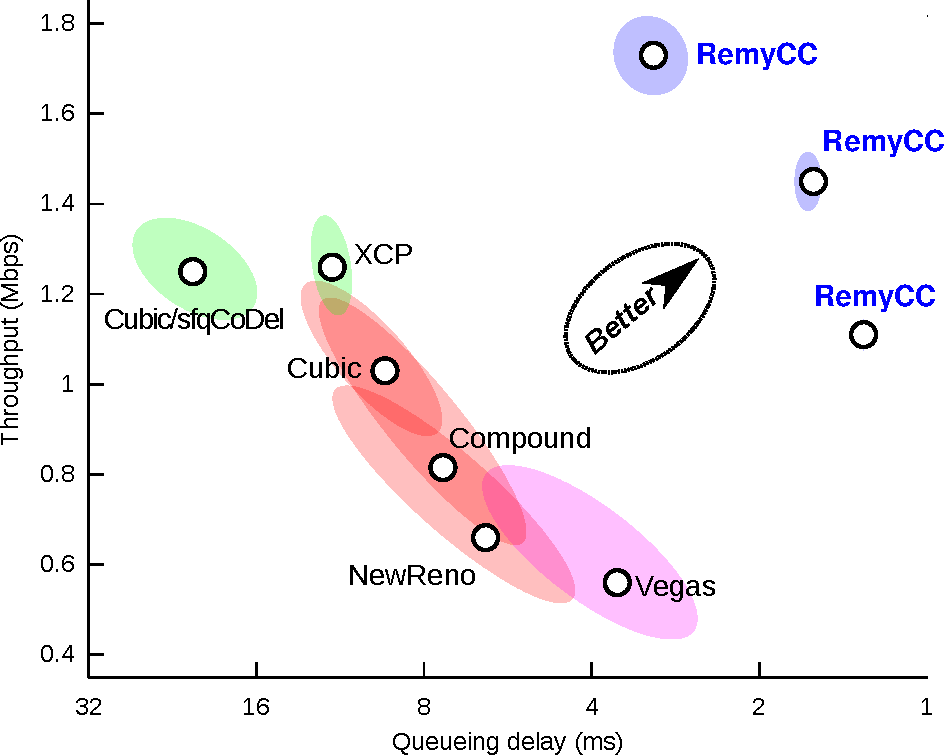
\includegraphics[width=0.8 \columnwidth]{eth8-annotated.pdf}
\def\svgwidth{0.8 \textwidth}\footnotesize\input{eth8-annotatedb.pdf_tex}
\end{center}
\end{minipage}

\newpage

More broadly, computer-generated protocols have led us to a style
of design where the value of information can be evaluated
empirically. We may give Remy access to a new congestion
signal---either a function of existing TCP acknowledgments from the
receiver, or based on a new source of information---and measure
how much the resulting congestion-control algorithm improves over the
status quo. Similarly, we can knock out an existing signal and rerun
Remy to measure how much the loss would hurt performance.

After investigating many candidate signals, we have ended up with
computer-generated algorithms that collect four congestion signals
(Section~\ref{ss:signals}). \textbf{None of these signals} is
collected by traditional TCP congestion-control schemes. Our
simulation experiments indicate each signal is individually valuable on
top of the other three.

\subsection{Windowing and pacing work well together}

Traditional congestion-control algorithms are window-based and
ack-clocked.~\cite{Srikant} Some proposed algorithms use
\emph{pacing}---transmitting packets according to an internal clock at
the sender---but the performance of these algorithms can display
counter-intuitive weaknesses.~\cite{understandingpacing}

After studying the behavior of Remy's algorithms and examining their
internal logic, we found they often behave as a fine-grained
hybrid of these two techniques, qualitatively different in behavior
than prior window- or pacing-based algorithms. In steady state, the
RemyCCs alternate between windowing and
pacing behavior. Within any interval that is at least 2 RTTs, some of
the algorithm's transmissions will have been gated by a windowing
constraint (waiting until the congestion window is larger than the
number of packets in flight), and some will have been gated by a
pacing constraint (waiting until the last packet transmitted was sent
long enough ago).

In practice, this hybrid behavior tends to produce quicker convergence to a
fair allocation of network resources when a flow starts or finishes
than traditional TCP-like schemes. We suspect there may be more to say
on the topic of ``windowing vs.~pacing'' if new algorithms similarly
attempt to use both techniques nearly concurrently.

\subsection{TCP-friendliness carries a benefit, but also a cost}

Congestion-control protocols are often evaluated for their
TCP-friendliness~\cite{friendlysurvey}, or in other words, for how
well they share a contended network resource with traditional TCP
flows as another TCP would.  By default, RemyCCs do not
play well with TCP on the same bottleneck---they are too deferential
and end up receiving less than their fair share.\footnote{RemyCCs
  generally try to keep standing queues small, both because we provide
  Remy with an objective that penalizes excess delay, but also because
  the shorter the queueing delay, the quicker the convergence time and
  the greater the throughput available to new flows. A long-running
  traditional TCP flow will work to fill queues until they overflow.}

This can be corrected, by telling Remy explicitly to assume a nonzero
risk that its algorithm may be contending with a traditional TCP
flow. In that case, the resulting RemyCCs do manage to claim their
fair share of the link (Figure~\ref{fig:tcpheterog}). But this
TCP-friendliness comes at a cost. By making the RemyCC more aggressive
in order to match up with TCP, the protocol ends up creating more
of a standing queue when it shares the network only
with other RemyCCs of the same type. From Figure~\ref{fig:tcphomog}:

\begin{center}
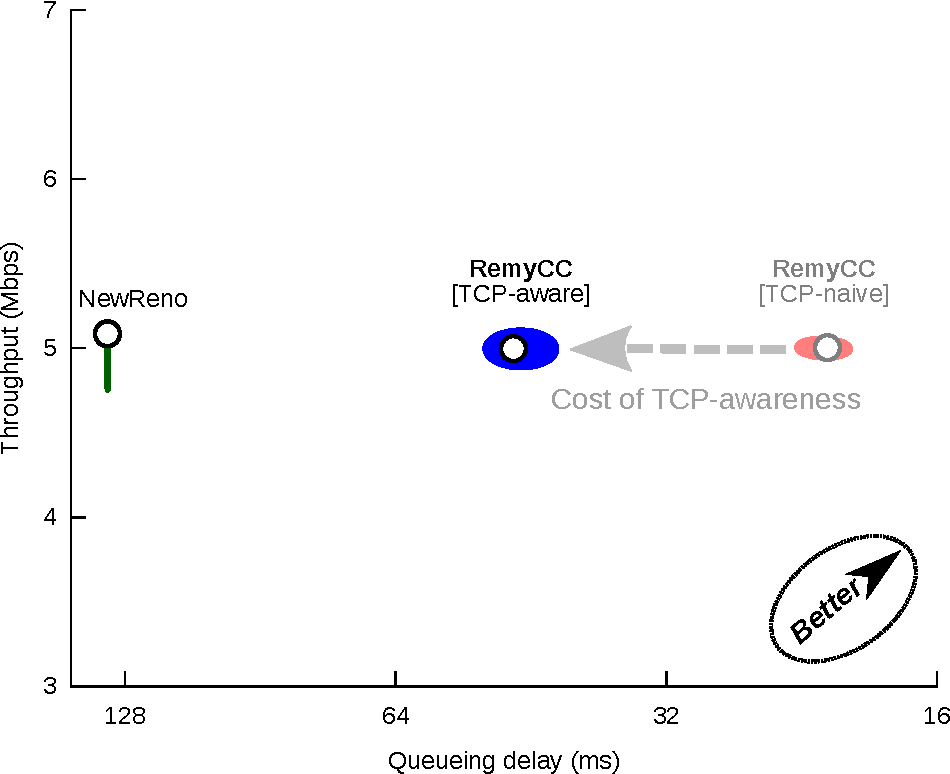
\includegraphics[width=0.75 \textwidth]{homo-3.pdf}
\end{center}

In other words, TCP-friendliness is a beneficial property \emph{when
  traditional TCP flows may be present on the same bottleneck}. But it
imposes a measurable cost in ``clean-slate'' designs. On internal networks
under the control of one entity, this may be worth taking into account.

\subsection{Assumptions about link rates and multiplexing are important}

We used Remy as a formalized model of the protocol-design process, to
ask rigorously: how faithfully do protocol designers really need to
understand the networks they design for?

We found that when modeling the network and link layers, it was
important for the designer's assumptions about \emph{some} network
parameters---the bottleneck link rate and the maximum degree of
multiplexing at the bottleneck---to include the true values of those
parameters.

In one experiment, we asked Remy to generate four different
congestion-control protocols, given different amounts of uncertainty
in the prior assumptions about the link rate: two-fold uncertainty,
ten-fold, hundred-fold, or thousand-fold. We then ran each protocol over a
broad range of actual link rates.

We found that performance fell dramatically when the link rate drifted
outside an algorithm's ``assumed'' range. It was possible for a
Remy-generated algorithm to outperform traditional algorithms over the
full thousand-fold range---but \textbf{only} when this possibility had
been included in the algorithm's prior assumptions. Algorithms with
more limited imagination fared poorly. From Figure~\ref{fig:breadth}:

\begin{center}
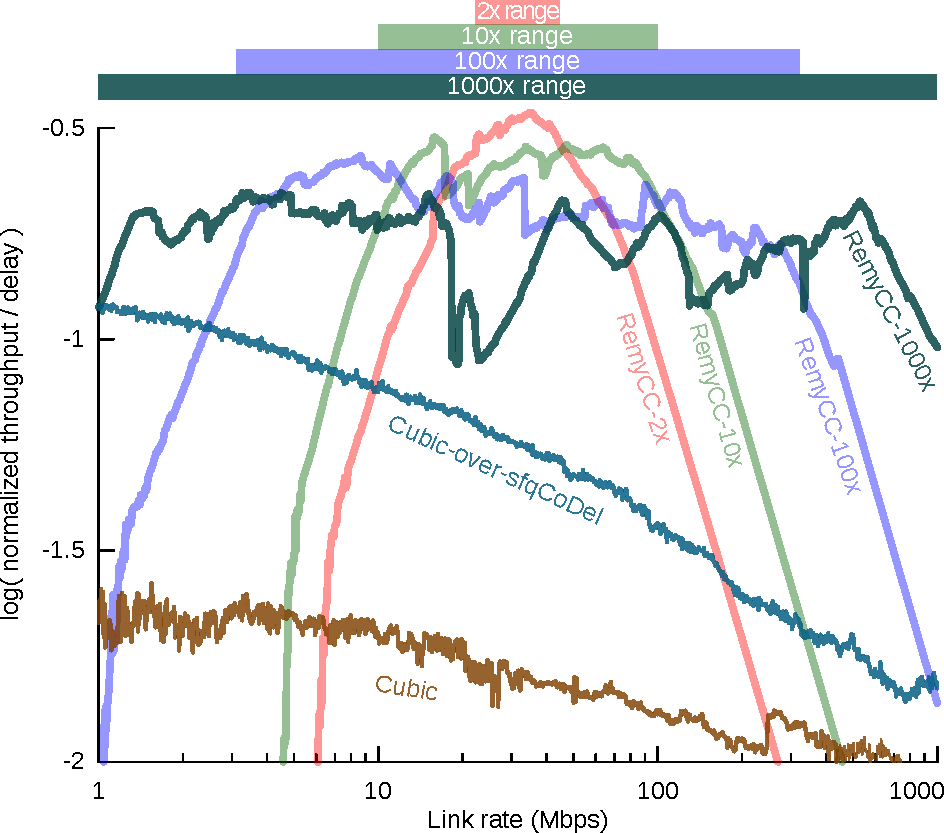
\includegraphics[width=0.75 \columnwidth]{oprange-manual.pdf}
\end{center}

The results suggest that human-generated protocols are also sensitive
to prior assumptions---the performance of Cubic-over-sfqCoDel trailed
off at higher link rates, suggesting this scheme may be making an implicit
assumption about the bandwidth-delay product that no longer holds at
such rates. However, it would be challenging to state explicitly the
assumptions of a mechanism like Cubic-over-sfqCoDel.

Among Remy-designed schemes, we also found considerable sensitivity to
prior assumptions about the maximum degree of multiplexing at a
bottleneck link. By contrast, we found less sensitivity to prior
assumptions about the expected distribution of round-trip times or the
topology of the network (Section~\ref{ss:topological}).

%\end{figure}

\section{Congestion control for all}

Since the 1980s, congestion control has been a well-studied topic in
the networking community. Its importance to the Internet may still be
growing. Google is putting congestion control in its Chrome Web
browser, as part of the QUIC project to send Web traffic over UDP and
to allocate limited network resources in a way that optimizes
application-specific objectives (e.g., the Web ``speed index'').

Netflix, said to account for the majority of Internet traffic in the
United States, is working on improving its congestion control in the
context of rate selection for progressive-download video, after
research findings that its existing algorithm could produce poor results.~\cite{huang2012confused}

Meanwhile, ``big data'' batch processing in specialized datacenters
continues to explode. Optimizing the communications of computers
connected by a datacenter switching fabric---again, in order to
achieve application-specific objectives---has drawn considerable
research and commercial effort~\cite{dctcp, pfabric}.

I believe that application needs and network behaviors will continue
to evolve as the Internet keeps growing and maturing. Congestion
control, and the transport layer generally, could adapt gracefully to
this innovation if they were merely a \emph{function} of a designer's
network assumptions and application-specific goals. Sprout and Remy
represent the first steps of showing what that would look
like.
